Simplify the following block diagram


\begin{center}
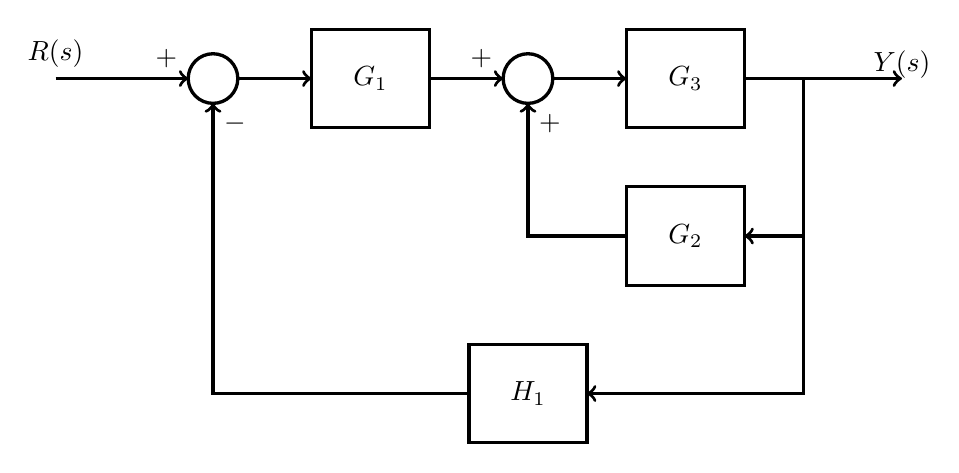
\begin{tikzpicture}[inner sep=0pt,outer sep=0pt,very thick,
sysblock/.style={draw,rectangle,inner sep=2pt,minimum width=1.5cm,minimum height=1.25cm,very thick}]
\draw (2,0) node[sysblock] (G1) {$G_{1}$};
\draw (6,-2) node[sysblock] (G2) {$G_{2}$};
\draw (0,0) node[draw,circle] (sum1) {$\rule{0pt}{18pt}$};
\draw (sum1) ++(.75,0) node[fill=black] (a) {};
\draw (4,0) node[draw,circle] (sum2) {$\rule{0pt}{18pt}$};
\draw (sum2) ++(.75,0) node[fill=black] (b) {};
\draw (6,0) node[sysblock] (G3) {$G_{3}$};
%\draw (8.5,0) node[draw,circle] (sum3) {$\rule{0pt}{18pt}$};
\draw (G3) ++(1.5,0) node[fill=black] (c) {};
\draw (G3) ++(2,0) node[fill=black] (d) {};
\draw (4,-4) node[sysblock] (H1) {$H_{1}$};

\draw[->] (-2,0) node[above=4pt] {$R(s)$} -- (sum1.180) node[above left=4pt] {$+$};
\draw[->] (sum1.0) -- (G1.180);
\draw[->] (G1.0) -- (sum2.180) node[above left=4pt] {$+$};
\draw[->] (sum2.0) -- (G3.180);
%\draw[->] (G3.0) -- (sum3.180);
%\draw[->] (sum3.0) -- ++(1,0) node[above] {$Y(s)$};
\draw[->] (G3.0) -- ++(2,0) node[above] {$Y(s)$};
\draw[->] (c) |- (G2.0);
\draw[->] (G2.180) -| (sum2.-90) node[below right=4pt] {$+$};
%\draw[->] (b) -- ++(0,1.5) -| (sum3.90) node[above right=4pt] {$-$};
\draw[->] (c) |- (H1.0) ;
\draw[->] (H1.180) -| (sum1.-90) node[below right=4pt] {$-$};
\end{tikzpicture}

\end{center}
